\documentclass[letter, 12pt, titlepage]{article}
\usepackage{graphicx}
\setlength{\parindent}{0pt}
\usepackage[left=1in,right=1in,top=1in,bottom=1in]{geometry}
\usepackage{listings}

\author{
	Dispoto, Brett\\
        \and
        Kamel, Adham\\
        \and
        Cai, Feiyu\\
}


\title{CS157A Team 2 \\ Database Design Documentation Revision \\
        \large A Book Reading and Review Web Application}

\begin{document}

  \maketitle
  	\section{Entity-Relationship Diagram}
	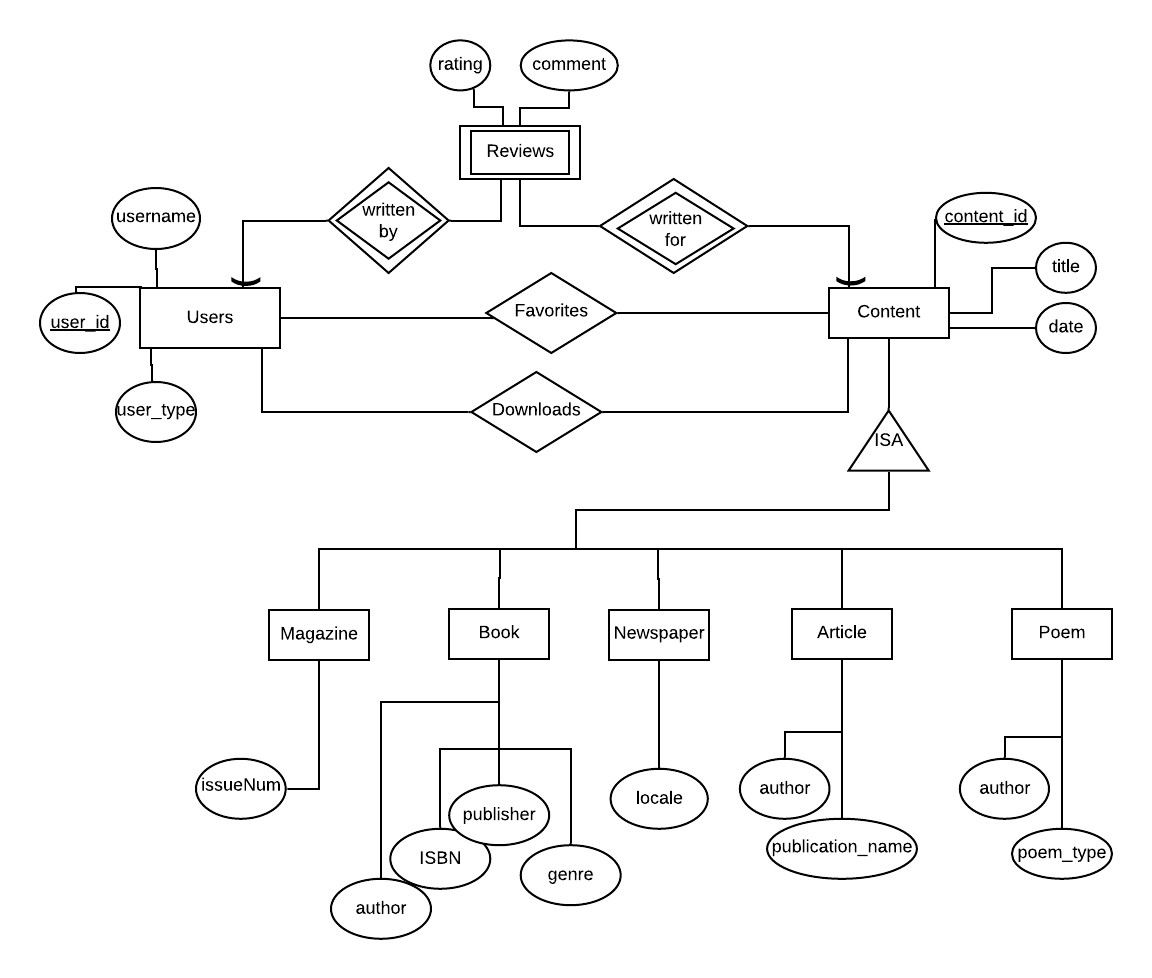
\includegraphics[scale=1]{erd-rev.png}
	\section{Database Schema}
		\begin{itemize}
			\item Users(\underline{user\_id}, username, use\_type)
			\item Reviews(\underline{user\_id}, \underline{content\_id}, rating, user\_comment)
			\item Favorites(\underline{user\_id}, \underline{content\_id})
			\item Downloads(\underline{user\_id}, \underline{content\_id} )
			\item Content(\underline{content\_id}, title, publish\_date)
			\item Article(\underline{conent\_id}, author, publication\_name)
			\item Magazine(\underline{content\_id}, issueNum)
			\item Book(\underline{content\_id}, ISBN, author, genre)
			\item Newspaper(\underline{content\_id}, locale)
			\item Poem(\underline{content\_id}, poem\_type, author)
		\end{itemize}
	\section{Database Tables}
		\subsection{Users}
			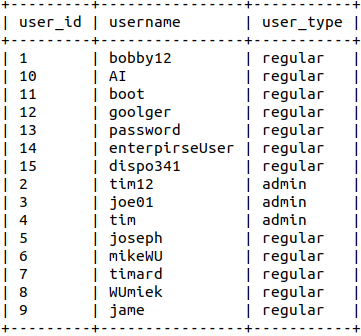
\includegraphics[scale=.5]{users.png}
		\subsection{Reviews}
			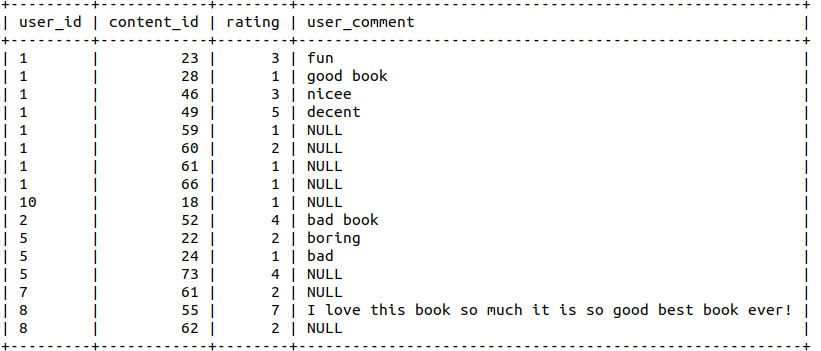
\includegraphics[scale=.5]{reviews.png}
		\subsection{Favorites}
			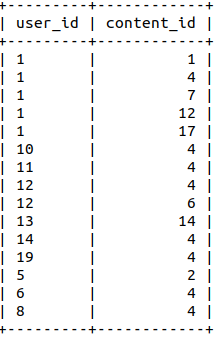
\includegraphics[scale=.5]{favorites.png}
		\subsection{Downloads}
			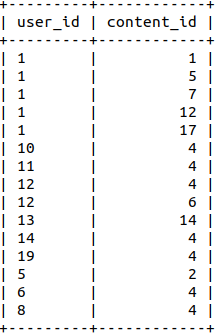
\includegraphics[scale=.5]{downloads.png}
		\subsection{Poem}
			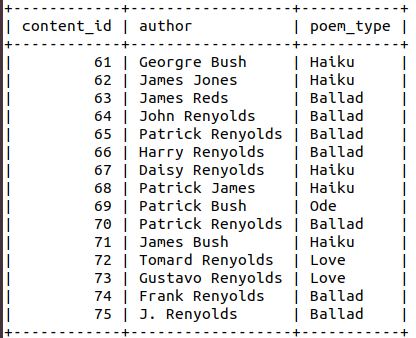
\includegraphics[scale=.45]{poem.png}
		\subsection{Content}
			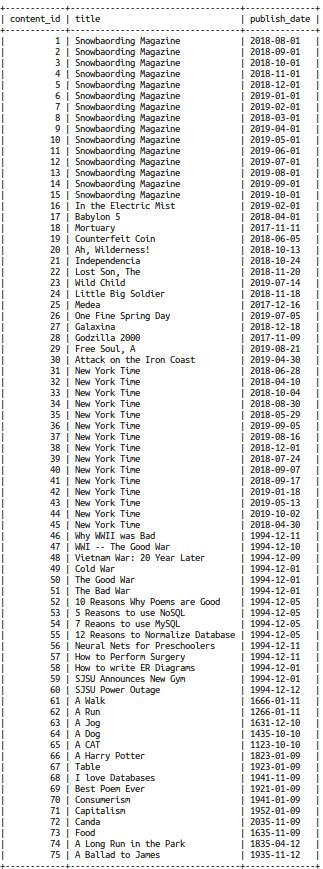
\includegraphics[scale=.7]{content.png}
		\subsection{Magazine}
			
\includegraphics[scale=.5]{magazine.png}
		\subsection{Article}
			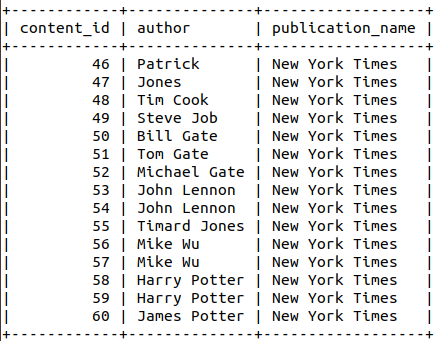
\includegraphics[scale=.5]{article.png}
		\subsection{Newspaper}
			
\includegraphics[scale=.5]{newspaper.png}
		\subsection{Book}
			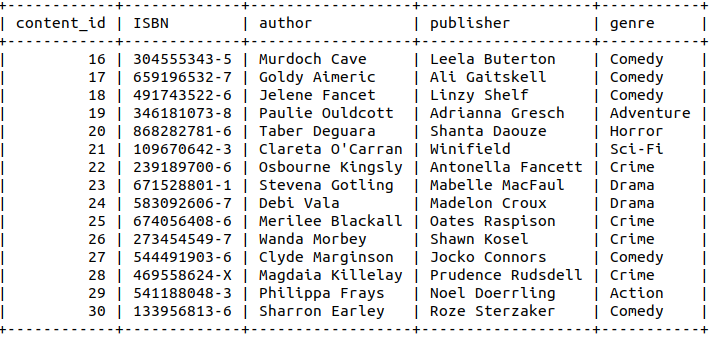
\includegraphics[scale=.5]{book.png}



	\section{Entities}
		\subsection{Users}
			Users are defined as those who have a valid account login for the website.
			The attributes for Users are as follows:
			\begin{itemize}
				\item type: A user can be of two types, admin or regular. Admins have special privileges
				\item username: The unique username by which a user logs into the web application
				\item userID: the unique identifier by which a user's information is tracked
			\end{itemize}
		\subsection{Content}
				Content comes in many forms. There are four subclasses of Content, but it possible that there exist an item that is only classifiable as Content and none of its subclasses. 
			
				The attributes for Content are as follows:
			\begin{itemize}
				\item content\_id: The unique content identifier
				\item title: The name/title of the content
				\item date: The date the content was published, if available
			\end{itemize}
			\subsection{Books}
				Books are a special case of Content. They have special attributes which sets them apart; however, books inherit the primary key from content. In addition, books have the following attributes:
			\begin{itemize}
				\item ISBN: the unique book ISBN number
				\item publisher: the publisher of the book
				\item author: The author of the book
				\item genre: the genre of the book
			\end{itemize}
			\subsection{Magazines}
				Magazines are a special case of Content. They have special attributes which sets them apart; however, magazines inherit the primary key from content. In addition, magazines have the following attributes:
			\begin{itemize}
				\item issueNum: the issue number of the magazine.
			\end{itemize}		
			\subsection{Newspapers} 
				Newspapers are a special case of Content. They have special attributes which sets them apart; however, Newspapers inherit the primary key from content. In addition, magazines have the following attributes:
			\begin{itemize}
				\item location: the locality of a Newspaper, if available.
				\item publication: the name of the newspaper publication
			\end{itemize}	
			\subsection{Articles}		
			Articles are standalone pieces of writing which may, in some cases, be significant enough to publish on the web application as it's own piece of media. Articles inherit the primary key from Content but have additional relationships, as described in the relationships section. Articles also have the following additional attributes:
			\begin{itemize}
				\item author: the author of the article
			\end{itemize}
		\subsection{Poems}		
			Poems are a specialized form of content, usually artistic in nature. Poems inherit the primary key from Content but have additional attributes, as described in the relationships section. Articles also have the following additional attributes:
			\begin{itemize}
				\item author: the author of the poem (if available)
				\item type: the type of poem (ballad, epic, prose, haiku, etc.)
			\end{itemize}
					
			\subsection{Reviews}
			Reviews are the way by which users rate their satisfaction with a particular piece of content. Reviews are a weak entity set due to the reliance on the primary keys from its relationships with User and Content, as described in the relationship section. Reviews consist of the following attributes:
			\begin{itemize}
				\item rating: the star rating given (out of 5)
				\item comment: the comment left in addition to the rating (optional)
			\end{itemize}

	\section{Relationships}
		\subsection{User Writes Reviews}
			A user (admin or regular) is the author of zero or many reviews. The weak entity set Review borrows the primary key username of User. This is a supporting relationship for the Review entity set.
		\subsection{Review Written for Content}
			A piece of content can obtain many reviews, but each review only belongs to one particular piece of content. The weak entity set Review borrows the primary key id from Content. This is a supporting relationship for the Review entity set.
		\subsection{User Favorites Content}
			A user can favorite content, which allows them to keep track of their favorite items. Content can be favorited by zero or many users. Users can favorite zero or many pieces of content.	
		\subsection{User Downloads Content}
			We would like to keep track of user's download history. A user can download zero or many pieces of content, and a piece of content may be downloaded by zero or many users.
\end{document}
